\documentclass[11pt]{article}
\usepackage[a4paper,margin=18mm]{geometry}
\usepackage{amsmath,amssymb}
\usepackage{booktabs}
\usepackage{tabularx}
\usepackage{enumitem}
\usepackage{xcolor}
\usepackage{microtype}
\usepackage[colorlinks=true,linkcolor=blue!50!black,urlcolor=blue!50!black]{hyperref}
\usepackage{tikz}
\usepackage{pgfplots}
\pgfplotsset{compat=1.18}
\usepgfplotslibrary{fillbetween}
\usetikzlibrary{positioning,arrows.meta,shapes.geometric,shapes.misc,calc,fit,backgrounds,decorations.pathreplacing}

\definecolor{blk}{HTML}{2C3E50}
\definecolor{acc}{HTML}{2980B9}
\definecolor{ok}{HTML}{27AE60}
\definecolor{warn}{HTML}{E67E22}
\definecolor{soft}{HTML}{EAF2F8}
\definecolor{soft2}{HTML}{FEF5E7}

\tikzset{
  >={Stealth[length=2.2mm]},
  block/.style={draw=blk, thick, rounded corners=2pt, fill=soft, minimum height=8mm,
                minimum width=15mm, align=center, font=\small},
  plant/.style={block, fill=warn!12, draw=warn!70!black},
  sum/.style={draw=blk, thick, circle, inner sep=0pt, minimum size=5mm, font=\footnotesize},
  sig/.style={font=\footnotesize\itshape},
  flow/.style={draw=acc, thick, rounded corners=3pt, fill=soft, align=center,
               font=\small, minimum height=8mm, inner sep=4pt, text width=34mm},
  dec/.style={draw=warn!80!black, thick, fill=soft2, align=center, font=\footnotesize,
              inner sep=3pt, rounded corners=7pt},
  l/.style={->, thick, draw=blk},
}
\newcommand{\diagram}[2][0.95]{\begin{center}\scalebox{#1}{#2}\end{center}}

\title{\textbf{Prior-art deep dive: how each multirotor autotuner works}\\[2pt]
\large Mechanism teardown for building an on-rig, GCS-driven PID tuner}
\author{Vayu GCS roadmap --- companion to \texttt{gcs-live-rig-tuning.md}}
\date{2026-06-16}

\begin{document}
\maketitle

\noindent\small Architecture facts (where the optimizer runs, excitation type,
in-flight vs.\ offline, openness) are source-cited and adversarially verified
(see the study). Inner algorithm details (model order, RLS, exact search rules)
are established but \emph{version-specific} --- confirm against current source
before copying constants. Diagrams are conceptual, not byte-exact.\normalsize

\tableofcontents

% ======================================================================
\section{Background: the cascaded attitude controller}
Every tuner below tunes pieces of the \emph{same} structure. A multirotor
attitude controller is a cascade of two nested loops: an outer \textbf{angle (P)}
loop that turns an attitude error into a rate setpoint, wrapped around a fast
inner \textbf{rate (PID + feedforward)} loop.

\diagram{%
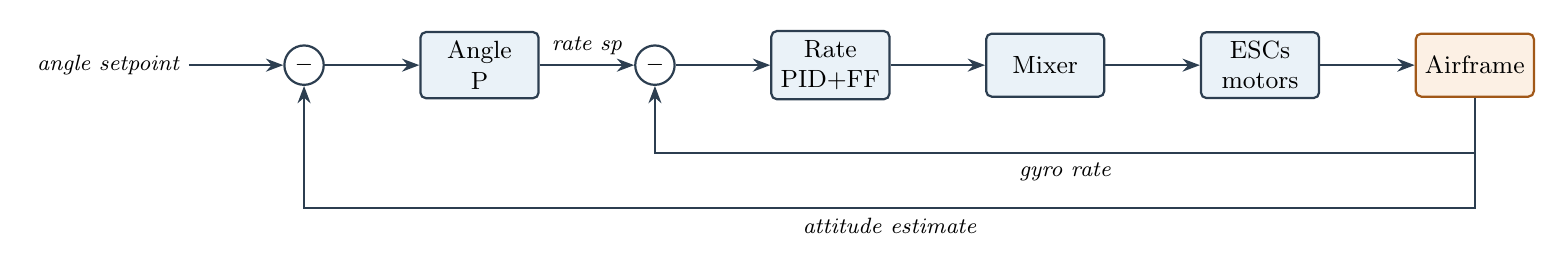
\begin{tikzpicture}[node distance=9mm and 12mm]
  \node[sig] (asp) {angle setpoint};
  \node[sum, right=of asp] (ae) {$-$};
  \node[block, right=of ae] (ap) {Angle\\P};
  \node[sum, right=of ap] (re) {$-$};
  \node[block, right=of re] (rp) {Rate\\PID+FF};
  \node[block, right=of rp] (mix) {Mixer};
  \node[block, right=of mix] (esc) {ESCs\\motors};
  \node[plant, right=of esc] (af) {Airframe};
  \draw[l] (asp) -- (ae);
  \draw[l] (ae) -- (ap);
  \draw[l] (ap) -- node[sig,above]{rate sp} (re);
  \draw[l] (re) -- (rp);
  \draw[l] (rp) -- (mix);
  \draw[l] (mix) -- (esc);
  \draw[l] (esc) -- (af);
  % gyro feedback (inner)
  \draw[l] (af.south) -- ++(0,-7mm) -| node[sig,pos=0.25,below]{gyro rate} (re.south);
  % attitude feedback (outer)
  \draw[l] (af.south) -- ++(0,-14mm) -| node[sig,pos=0.25,below]{attitude estimate} (ae.south);
\end{tikzpicture}}

\begin{itemize}[leftmargin=*,nosep]
\item \textbf{Inner = rate PID} (runs at the gyro/loop rate, hundreds of Hz--kHz):
$K_p,K_i,K_d$ + feedforward + a gyro low-pass. Dominates ``feel''; this is where
instability/oscillation lives.
\item \textbf{Outer = angle P}: only active in stabilize/angle mode. In acro/rate
mode only the inner loop runs --- which is why we tune \emph{per mode}.
\item \textbf{Tune rate before angle:} the outer loop assumes a well-behaved inner
loop.
\end{itemize}

Physically, ``tuning'' means: track a commanded change \emph{fast} (high
bandwidth) but without sustained oscillation, overshoot, or motor ``chatter''
(high-frequency $D$-noise amplification). Two paradigms cover everything:

\diagram[1.0]{%
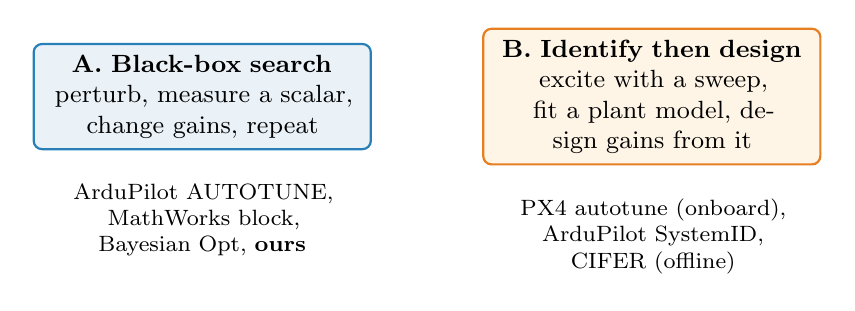
\begin{tikzpicture}[node distance=6mm and 14mm]
  \node[flow,fill=soft,draw=acc,text width=40mm] (a) {\textbf{A. Black-box search}\\perturb, measure a scalar, change gains, repeat};
  \node[flow,fill=soft2,draw=warn,text width=40mm, right=of a] (b) {\textbf{B. Identify then design}\\excite with a sweep, fit a plant model, design gains from it};
  \node[font=\footnotesize, below=3mm of a, text width=42mm, align=center] {ArduPilot AUTOTUNE, MathWorks block,\\ Bayesian Opt, \textbf{ours}};
  \node[font=\footnotesize, below=3mm of b, text width=42mm, align=center] {PX4 autotune (onboard),\\ ArduPilot SystemID, CIFER (offline)};
\end{tikzpicture}}

% ======================================================================
\section{ArduCopter AUTOTUNE --- onboard iterative twitch search (Paradigm A)}
\textbf{Source:} \url{https://ardupilot.org/copter/docs/autotune.html}

\paragraph{Setup.} Fly to a safe altitude in AltHold/Loiter in calm air, engage
AUTOTUNE via an RC switch, hold position with a hand on the sticks.
\texttt{AUTOTUNE\_AGGR} ($\approx$0.05--0.10) trades responsiveness vs.\ overshoot.

\paragraph{Control mechanics.} A brief commanded \textbf{rate step (``twitch'')}
is injected into the rate-loop setpoint of the axis under test; the FC watches the
gyro response and reads three features: peak rate, overshoot, and
bounce-back/ringing.

\diagram[0.92]{%
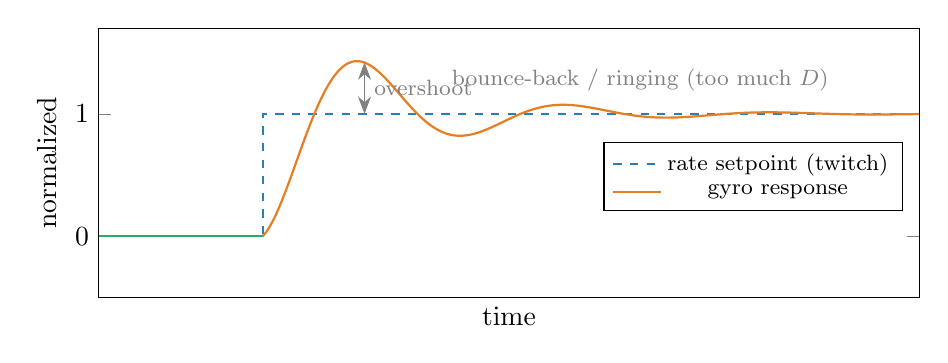
\begin{tikzpicture}
\begin{axis}[width=12cm,height=5cm,xlabel={time},ylabel={normalized},
  xtick=\empty, ytick={0,1}, ymin=-0.5, ymax=1.7, xmin=0, xmax=5,
  legend style={font=\footnotesize,at={(0.98,0.45)},anchor=east},
  every axis plot/.append style={thick}]
  \addplot[acc,dashed] coordinates {(0,0)(1,0)(1,1)(5,1)};
  \addlegendentry{rate setpoint (twitch)}
  \addplot[warn,domain=1:5,samples=200] {1-exp(-1.4*(x-1))*cos(deg(5*(x-1)))};
  \addlegendentry{gyro response}
  \addplot[ok,domain=0:1] {0};
  \draw[<->,gray] (axis cs:1.62,1.0) -- node[right,font=\footnotesize]{overshoot} (axis cs:1.62,1.42);
  \node[font=\footnotesize,gray] at (axis cs:3.3,1.28) {bounce-back / ringing (too much $D$)};
\end{axis}
\end{tikzpicture}}

\paragraph{Algorithm (bracketing search, no model).} Per axis: raise rate-$D$
until the response just rings, back off; raise rate-$P$ to a target response; set
angle-$P$ from the achieved bandwidth with an \texttt{AGGR} margin.

\diagram[0.9]{%
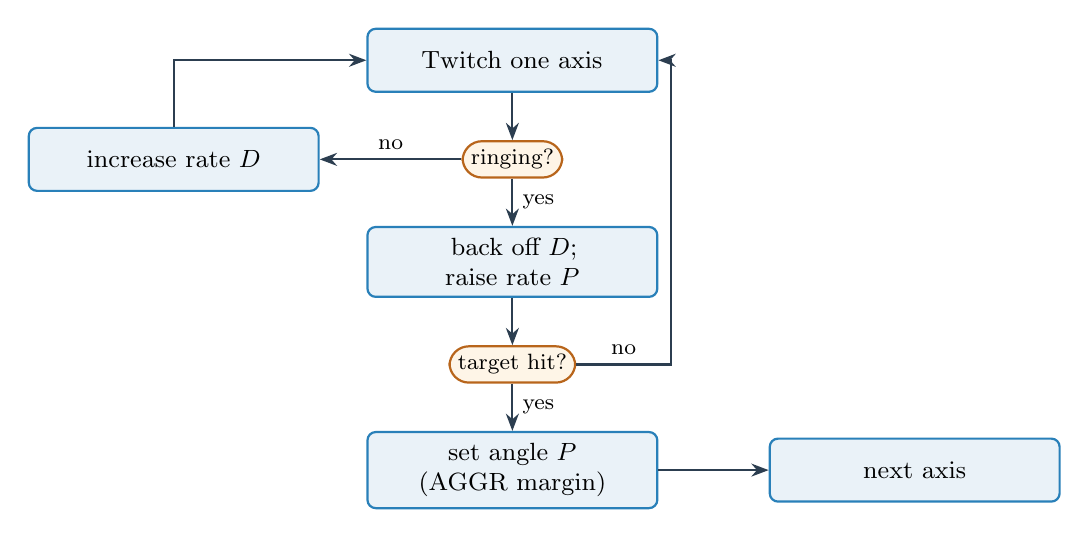
\begin{tikzpicture}[node distance=6mm and 10mm]
  \node[flow] (s) {Twitch one axis};
  \node[dec, below=of s] (q) {ringing?};
  \node[flow, left=18mm of q] (incd) {increase rate $D$};
  \node[flow, below=of q] (bp) {back off $D$;\\ raise rate $P$};
  \node[dec, below=of bp] (q2) {target hit?};
  \node[flow, below=of q2] (ag) {set angle $P$ (AGGR margin)};
  \node[flow, right=14mm of ag] (nx) {next axis};
  \draw[l] (s) -- (q);
  \draw[l] (q) -- node[above,font=\footnotesize]{no} (incd);
  \draw[l] (incd) |- (s);
  \draw[l] (q) -- node[right,font=\footnotesize]{yes} (bp);
  \draw[l] (bp) -- (q2);
  \draw[l] (q2.east) -- node[above,font=\footnotesize]{no} ++(12mm,0) |- (s);
  \draw[l] (q2) -- node[right,font=\footnotesize]{yes} (ag);
  \draw[l] (ag) -- (nx);
\end{tikzpicture}}

\paragraph{Safety.} Original gains preserved; moving the sticks hands control back
instantly; disarm/exit \emph{reverts} unless the operator explicitly saves
(land + low throttle). Self-aborts on excessive attitude error.

\paragraph{Correctness / comms.} No model --- convergence is to a target rate
response per axis; the real test is the operator's post-tune flight. GCS only sets
params (MAVLink \texttt{PARAM\_SET}); results persisted on the FC. \textbf{GPLv3.}

\paragraph{Lift for ours.} The twitch + per-axis feature extraction is the
ancestor of our doublet rollout/cost; we move the \emph{search} to the GCS and
replace ``save on landing'' with explicit GCS Apply. Stick-override $\to$ our
operator gesture.

% ======================================================================
\section{ArduCopter SystemID --- chirp + offline model/PID design (Paradigm B)}
\textbf{Sources:} \url{https://ardupilot.org/copter/docs/systemid-model-development.html},
\url{https://ardupilot.org/copter/docs/common-systemid-mode-operation.html}

\paragraph{Control mechanics.} A frequency-sweep (\textbf{chirp}) is
\emph{superimposed on the mixer input} of the chosen axis via \texttt{SID\_AXIS}
(10/11/12 = roll/pitch/yaw), generated onboard.

\diagram[0.92]{%
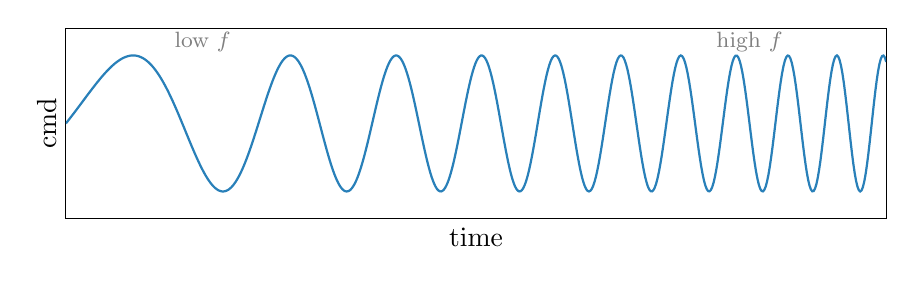
\begin{tikzpicture}
\begin{axis}[width=12cm,height=4cm,xlabel={time},ylabel={cmd},xtick=\empty,ytick=\empty,
  xmin=0,xmax=6,ymin=-1.4,ymax=1.4]
  \addplot[acc,thick,domain=0:6,samples=600] {sin(deg(2*pi*(0.4*x+0.22*x*x)))};
  \node[font=\footnotesize,gray] at (axis cs:1.0,1.2){low $f$};
  \node[font=\footnotesize,gray] at (axis cs:5.0,1.2){high $f$};
\end{axis}
\end{tikzpicture}}

\paragraph{Algorithm (two offline stages).} (1) Transform logged $u(t),y(t)$ to
the frequency domain; fit a plant transfer function whose parameters maximize the
fit to the measured frequency response. (2) Use the model to optimize the PID.

\diagram[0.9]{%
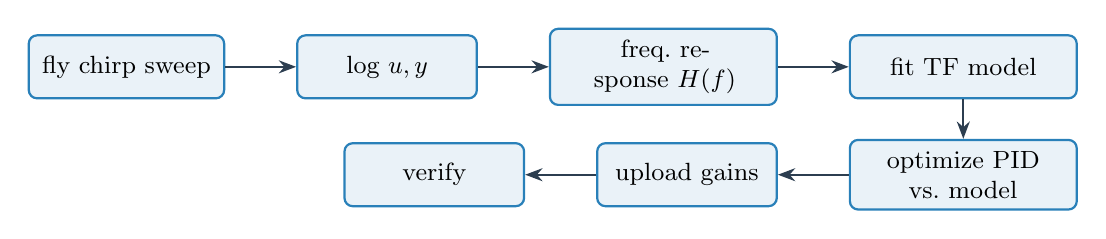
\begin{tikzpicture}[node distance=5mm and 9mm]
  \node[flow,text width=22mm] (a){fly chirp sweep};
  \node[flow,text width=20mm,right=of a] (b){log $u,y$};
  \node[flow,text width=26mm,right=of b] (c){freq.\ response $H(f)$};
  \node[flow,text width=26mm,right=of c] (d){fit TF model};
  \node[flow,text width=26mm,below=of d] (e){optimize PID vs.\ model};
  \node[flow,text width=20mm,left=of e] (f){upload gains};
  \node[flow,text width=20mm,left=of f] (g){verify};
  \draw[l](a)--(b); \draw[l](b)--(c); \draw[l](c)--(d); \draw[l](d)--(e);
  \draw[l](e)--(f); \draw[l](f)--(g);
\end{tikzpicture}}

\paragraph{Lift for ours.} Proof that an \textbf{FC-side chirp at the
mixer/setpoint axis} is a sound injection point (= our ``override the axis
setpoint''). \textbf{GPLv3.}

% ======================================================================
\section{PX4 \texttt{mc\_autotune} --- fully onboard sys-ID + gain calc}
\textbf{Sources:} \url{https://docs.px4.io/main/en/config/autotune_mc},
\url{https://docs.px4.io/main/en/msg_docs/AutotuneAttitudeControlStatus}

\paragraph{Setup \& mechanics.} The vehicle must be \emph{flying} in an
altitude-stabilized mode (not a bench); QGC triggers it. The stack applies a small
per-axis disturbance (a doublet) and records filtered input $u_{\text{filt}}$
(normalized torque setpoint) and output $y_{\text{filt}}$ (angular velocity).

\diagram{%
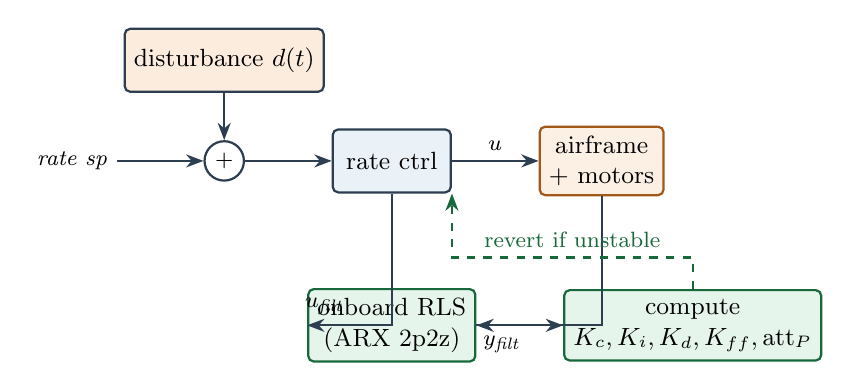
\begin{tikzpicture}[node distance=8mm and 11mm]
  \node[sig] (rsp){rate sp};
  \node[sum,right=of rsp] (add){$+$};
  \node[block,above=6mm of add,fill=warn!15] (d){disturbance $d(t)$};
  \node[block,right=of add] (rc){rate ctrl};
  \node[plant,right=of rc] (af){airframe\\+ motors};
  \node[block,below=12mm of rc,fill=ok!12,draw=ok!60!black] (id){onboard RLS\\(ARX 2p2z)};
  \node[block,right=of id,fill=ok!12,draw=ok!60!black] (gc){compute\\$K_c,K_i,K_d,K_{ff},\text{att}_P$};
  \draw[l](rsp)--(add); \draw[l](d)--(add); \draw[l](add)--(rc);
  \draw[l](rc)-- node[sig,above]{$u$} (af);
  \draw[l](rc.south) |- node[sig,pos=0.9,above]{$u_{\text{filt}}$} (id.west);
  \draw[l](af.south) |- node[sig,pos=0.9,below]{$y_{\text{filt}}$} (id.east);
  \draw[l](id)--(gc);
  \draw[l,dashed,ok!60!black](gc.north) -- ++(0,4mm) -| node[pos=0.25,above,font=\footnotesize]{revert if unstable} (rc.south east);
\end{tikzpicture}}

\paragraph{Algorithm.} Identify a low-order discrete \textbf{ARX} model
($\approx$2-pole/2-zero) by \textbf{recursive least squares}, conceptually
\[
  y[k] = -a_1 y[k-1] - a_2 y[k-2] + b_1 u[k-1] + b_2 u[k-2],
\]
with $\hat\theta=(a_1,a_2,b_1,b_2)$ updated each sample and a covariance that
shrinks as evidence accumulates. The uORB message exposes \texttt{coeff}
($a,b$), \texttt{coeff\_var} (confidence), and a \textbf{fitness}. From the model,
gains are computed analytically (target crossover/phase margin). Axes run
sequentially roll$\to$pitch$\to$yaw.

\diagram[0.95]{%
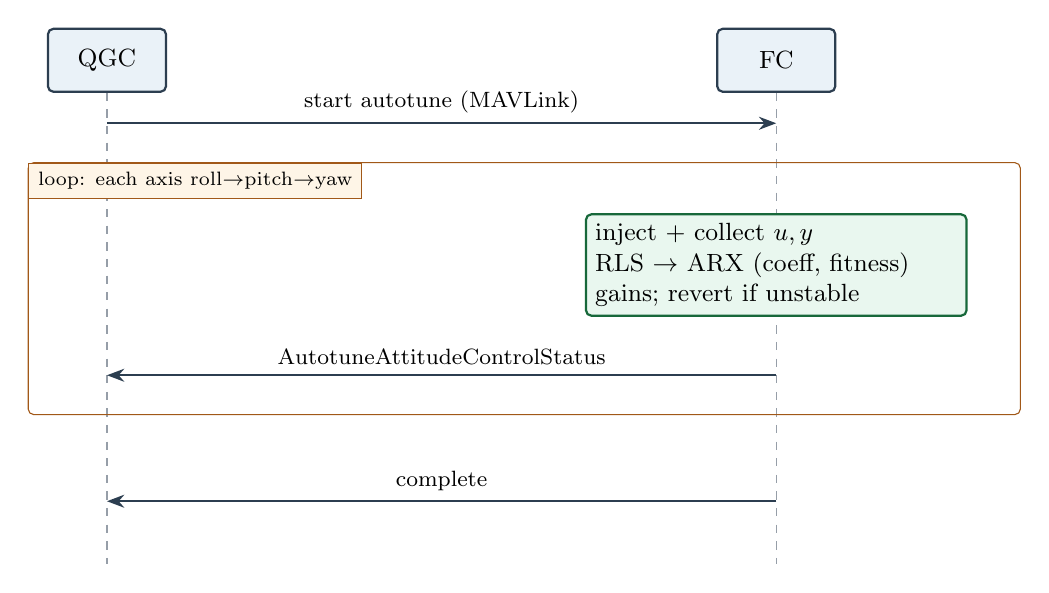
\begin{tikzpicture}[font=\footnotesize]
  \node[block] (q) at (0,0) {QGC};
  \node[block] (f) at (8.5,0) {FC};
  \draw[dashed,blk!50] (q.south) -- (0,-6.4);
  \draw[dashed,blk!50] (f.south) -- (8.5,-6.4);
  \draw[l] (0,-0.8) -- node[above]{start autotune (MAVLink)} (8.5,-0.8);
  % loop frame
  \draw[warn!70!black,rounded corners=2pt] (-1.0,-1.3) rectangle (11.6,-4.5);
  \node[draw=warn!70!black,fill=soft2,font=\scriptsize,anchor=north west] at (-1.0,-1.3) {loop: each axis roll$\to$pitch$\to$yaw};
  % FC activation box
  \node[block,fill=ok!10,draw=ok!60!black,align=left,text width=46mm] (act) at (8.5,-2.6)
    {inject + collect $u,y$\\ RLS $\to$ ARX (coeff, fitness)\\ gains; revert if unstable};
  \draw[l] (8.5,-4.0) -- node[above]{AutotuneAttitudeControlStatus} (0,-4.0);
  \draw[l] (8.5,-5.6) -- node[above]{complete} (0,-5.6);
\end{tikzpicture}}

\paragraph{Lift for ours.} Strongest precedent for \textbf{FC-side excitation +
onboard scoring} (PX4 computes a fitness onboard = our FC-side cost). Difference:
PX4 also computes \emph{gains} onboard from a model; we keep the iterative gain
choice on the GCS and skip the model. \textbf{BSD-3.}

% ======================================================================
\section{PX4 manual / step-input tuning --- the human baseline}
\textbf{Source:} \url{https://docs.px4.io/main/en/config_mc/pid_tuning_guide_multicopter}.
No optimizer: hover, give a fast \textbf{stick step}, observe oscillation/overshoot,
\emph{land before changing a parameter}, repeat. The ``land between changes'' rule
is the safety system. Our rig + operator-gated re-stabilize replaces that cadence.

% ======================================================================
\section{CIFER + CONDUIT / Simulink --- offline frequency-domain pipeline}
\textbf{Sources:}
\url{https://arxiv.org/pdf/1508.04886}, \url{https://www.sjsu.edu/researchfoundation/docs/AHS_2015_Wei.pdf},
\url{https://arxiv.org/pdf/0804.3881}

\paragraph{Setup.} Fly frequency sweeps in hover, axis by axis (human-piloted or,
better, autopilot-generated --- a human cannot cleanly cover the whole band).
Analysis is entirely offline.

\diagram[0.88]{%
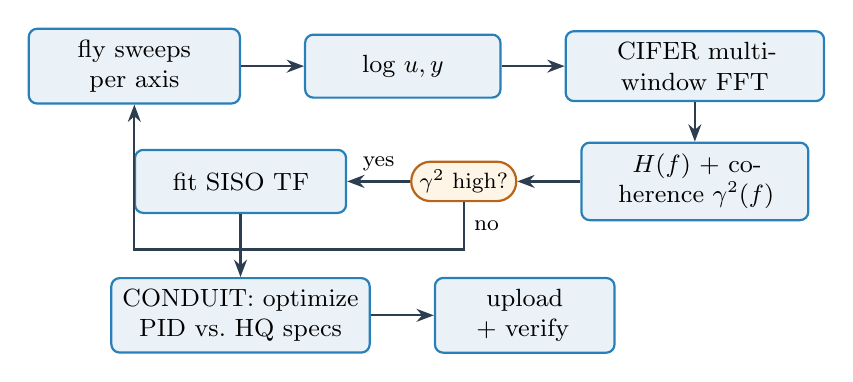
\begin{tikzpicture}[node distance=5mm and 8mm]
  \node[flow,text width=24mm] (a){fly sweeps per axis};
  \node[flow,text width=22mm,right=of a] (b){log $u,y$};
  \node[flow,text width=30mm,right=of b] (c){CIFER multi-window FFT};
  \node[flow,text width=26mm,below=of c] (d){$H(f)$ + coherence $\gamma^2(f)$};
  \node[dec,left=of d] (g){$\gamma^2$ high?};
  \node[flow,text width=24mm,left=of g] (e){fit SISO TF};
  \node[flow,text width=30mm,below=8mm of e] (f){CONDUIT: optimize PID vs.\ HQ specs};
  \node[flow,text width=20mm,right=of f] (u){upload + verify};
  \draw[l](a)--(b);\draw[l](b)--(c);\draw[l](c)--(d);\draw[l](d)--(g);
  \draw[l](g)-- node[above,font=\footnotesize]{yes} (e);
  \draw[l](g.south)-- node[right,font=\footnotesize]{no} ++(0,-6mm) -| (a.south);
  \draw[l](e)--(f);\draw[l](f)--(u);
\end{tikzpicture}}

\paragraph{Core concepts.} The frequency response $H(f)$ is a Bode plot of the
airframe; a sweep measures the whole curve at once. The \textbf{coherence}
\[
  \gamma^2(f)=\frac{|S_{xy}(f)|^2}{S_{xx}(f)\,S_{yy}(f)} \in [0,1]
\]
is the \emph{data-quality gate}: $\gamma^2\!\approx\!1$ means the output is
linearly explained by the input (low noise); bands with $\gamma^2<\sim0.6$ are
dropped. CONDUIT then optimizes the PID against handling-qualities specs.

\paragraph{Lift for ours.} \textbf{Coherence as a rollout-quality gate} --- reject
a noisy/gappy pass before scoring. Tools proprietary; method fully published.

% ======================================================================
\section{MathWorks Closed-Loop PID Autotuner}
\textbf{Source:} \url{https://www.mathworks.com/help/slcontrol/ug/pid-controller-tuning-for-a-uav-quadcopter.html}.
A Simulink block in the loop (deployable to hardware) that injects \textbf{sinusoidal
perturbations at the controller output} (actuator command), so the existing
controller keeps the craft stable \emph{during} the experiment; it estimates the
plant FRF in closed loop and computes gains in the block.

\diagram{%
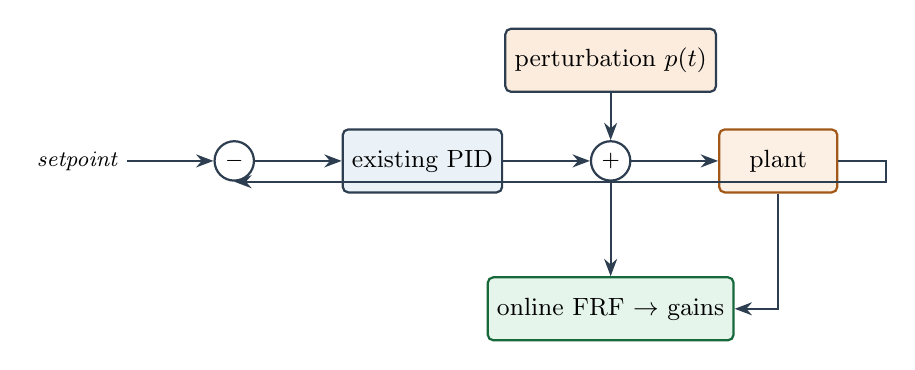
\begin{tikzpicture}[node distance=8mm and 11mm]
  \node[sig](sp){setpoint};
  \node[sum,right=of sp](e){$-$};
  \node[block,right=of e](pid){existing PID};
  \node[sum,right=of pid](add){$+$};
  \node[block,above=6mm of add,fill=warn!15](p){perturbation $p(t)$};
  \node[plant,right=of add](pl){plant};
  \node[block,below=12mm of add,fill=ok!12,draw=ok!60!black](est){online FRF $\to$ gains};
  \draw[l](sp)--(e);\draw[l](e)--(pid);\draw[l](pid)--(add);\draw[l](p)--(add);\draw[l](add)--(pl);
  \draw[l](pl.east)-- ++(6mm,0) |- (e.south);
  \draw[l](add.south)--(est.north -| add.south);
  \draw[l](pl.south) |- (est.east);
\end{tikzpicture}}

\paragraph{Lift for ours.} ``Perturb at the controller output, identify in closed
loop'' is a fallback excitation point if clean \emph{setpoint} override is awkward
on the FC. \textbf{Proprietary.}

% ======================================================================
\section{Safe Bayesian Optimization on hardware (Berkenkamp et al.)}
\textbf{Source:} \url{https://las.inf.ethz.ch/files/berkenkamp16safe.pdf}.
The \textbf{closest architectural cousin}: an external optimizer proposes candidate
controller parameters, each is run as a real closed-loop trial, a scalar
performance (and a safety value) is measured, and the optimizer picks the next ---
exactly our GCS-as-optimizer / FC-evaluates-a-pass loop, minus the rig.

\diagram[0.9]{%
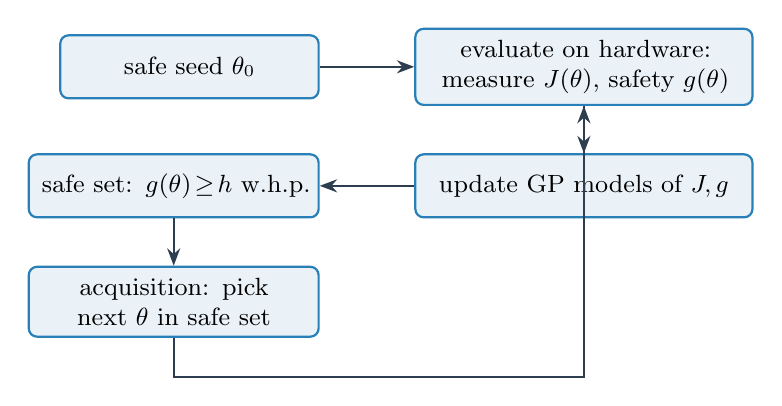
\begin{tikzpicture}[node distance=6mm and 12mm]
  \node[flow,text width=30mm] (s){safe seed $\theta_0$};
  \node[flow,text width=40mm,right=of s] (ev){evaluate on hardware: measure $J(\theta)$, safety $g(\theta)$};
  \node[flow,text width=40mm,below=of ev] (gp){update GP models of $J,g$};
  \node[flow,text width=34mm,left=of gp] (sa){safe set: $g(\theta)\!\ge\!h$ w.h.p.};
  \node[flow,text width=34mm,below=of sa] (ac){acquisition: pick next $\theta$ in safe set};
  \draw[l](s)--(ev);\draw[l](ev)--(gp);\draw[l](gp)--(sa);\draw[l](sa)--(ac);
  \draw[l](ac.south)-- ++(0,-5mm) -| (ev.south);
\end{tikzpicture}}

\paragraph{Core idea.} A Gaussian Process models $J(\theta)$ with a
\textbf{mean $\pm$ uncertainty} from only a few real trials; \textbf{SafeOpt} only
evaluates $\theta$ whose safety $g(\theta)$ stays above a threshold \emph{with high
probability}, expanding the safe region cautiously and never knowingly trying a
destabilizing gain.

\diagram[0.92]{%
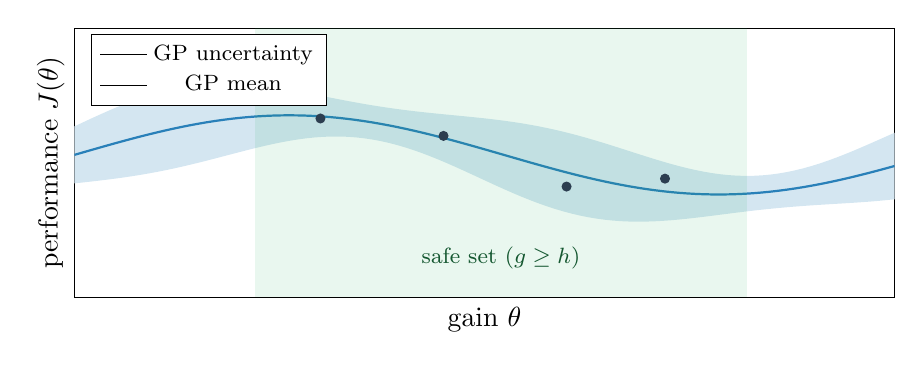
\begin{tikzpicture}
\begin{axis}[width=12cm,height=5cm,xlabel={gain $\theta$},ylabel={performance $J(\theta)$},
  xtick=\empty,ytick=\empty,xmin=0,xmax=10,ymin=-0.2,ymax=1.5,
  legend style={font=\footnotesize,at={(0.02,0.98)},anchor=north west}]
  % uncertainty band
  \addplot[name path=up,draw=none,domain=0:10,samples=100]{0.7+0.25*sin(deg(0.6*x))+0.18*(1+0.4*sin(deg(1.3*x)))};
  \addplot[name path=lo,draw=none,domain=0:10,samples=100]{0.7+0.25*sin(deg(0.6*x))-0.18*(1+0.4*sin(deg(1.3*x)))};
  \addplot[acc!20]fill between[of=up and lo]; \addlegendentry{GP uncertainty}
  \addplot[acc,thick,domain=0:10,samples=100]{0.7+0.25*sin(deg(0.6*x))}; \addlegendentry{GP mean}
  % safe region shading
  \fill[ok,opacity=0.10] (axis cs:2.2,-0.2) rectangle (axis cs:8.2,1.5);
  \node[font=\footnotesize,ok!50!black] at (axis cs:5.2,0.05){safe set ($g\ge h$)};
  % samples
  \addplot[only marks,mark=*,mark size=1.6pt,blk] coordinates {(3,0.93)(4.5,0.82)(6,0.5)(7.2,0.55)};
\end{axis}
\end{tikzpicture}}

\paragraph{Lift for ours.} If the reused SITL optimizer struggles with real noise,
\textbf{SafeOpt / Bayesian optimization is the prime candidate}: sample-efficient
(few slow rig rollouts) and safety-constrained (won't probe known-bad gains). We
keep the rig as the hard safety net; SafeOpt adds a soft, data-driven one.

% ======================================================================
\section{Adjacent systems (not closed-loop PID tuners)}
\textbf{Thrust stands (RCbenchmark / Tyto Robotics)} ---
\url{https://www.tytorobotics.com/pages/rcbenchmark-software} --- characterize a
single motor+prop (thrust/torque/RPM/current/efficiency), \emph{not} airframe PID.
Use them to feed real motor/prop constants into the SITL model so sim-tuned gains
transfer better. \textbf{Data-driven param-ID + RL} (Eschmann/Albani/Loianno 2024,
\url{https://arxiv.org/pdf/2404.07837}) identifies inertia/thrust/motor-delay from
$\sim$73\,s of free flight, then trains an RL policy --- free flight, learned
controller, not classical PID. \textbf{Betaflight}: no built-in closed-loop
autotuner (general; not source-verified) --- presets, filters, manual + sliders.

% ======================================================================
\section{Side-by-side mechanics}
\begin{center}\small
\begin{tabularx}{\linewidth}{@{}lXXll@{}}
\toprule
System & excitation / injected at & optimizer & safety net & data check\\
\midrule
ArduPilot AUTOTUNE & rate twitch @ rate setpoint & \textbf{FC} & stick override, revert & response features\\
ArduPilot SystemID & chirp @ mixer input & \textbf{offline PC} & pilot override & FRF fit\\
PX4 autotune & doublet @ torque setpoint & \textbf{FC} (RLS) & revert-unstable, alt-hold & fitness + variance\\
CIFER/CONDUIT & sweep @ pilot/AP stick & \textbf{offline PC} & safety pilot & \textbf{coherence}\\
MathWorks block & sinusoids @ ctrl output & \textbf{in block} & closed-loop stays stable & FRF margins\\
Safe BayesOpt & per-candidate trial & \textbf{external/host} & \textbf{GP safe set} & GP variance\\
\textbf{Ours} & doublet+chirp @ \textbf{setpoint (FC)} & \textbf{GCS} & \textbf{rig + operator gesture} & add coherence-style gate\\
\bottomrule
\end{tabularx}
\end{center}

\section{The composite ``ideal'' for our build}
\begin{itemize}[leftmargin=*,nosep]
\item \textbf{Excitation:} FC-generated doublet/chirp at the \emph{setpoint}
(ArduPilot SystemID injection point) --- jitter-immune, loop-rate exact.
\item \textbf{Score:} onboard cost (PX4 precedent) from FC-paired
setpoint/measured; add a coherence/gap quality gate (CIFER).
\item \textbf{Optimizer:} start with the SITL search; if real noise defeats it,
switch to \textbf{SafeOpt/Bayesian} (Berkenkamp).
\item \textbf{Safety:} mechanical rig (hard) + operator-gesture abort (ArduPilot)
+ revert-to-committed on exit (PX4/ArduPilot) + GCS Apply-with-confirmation.
\item \textbf{Genuinely new (no template):} the GCS-optimizer / FC-executor split,
and the constrained-rig closed-loop rollout --- design from first principles.
\end{itemize}

\end{document}
